\textbf{PROBLEMA 1}
\vspace{20px}

Considere un disco metálico horizontal (A) de radio $a$ y de espesor despreciable tal y como se muestra en
la figura. El disco está conectado a un generador de tensión $V_0$. Para un punto P en el eje $z$ del disco y sobre
este,

\begin{center}
    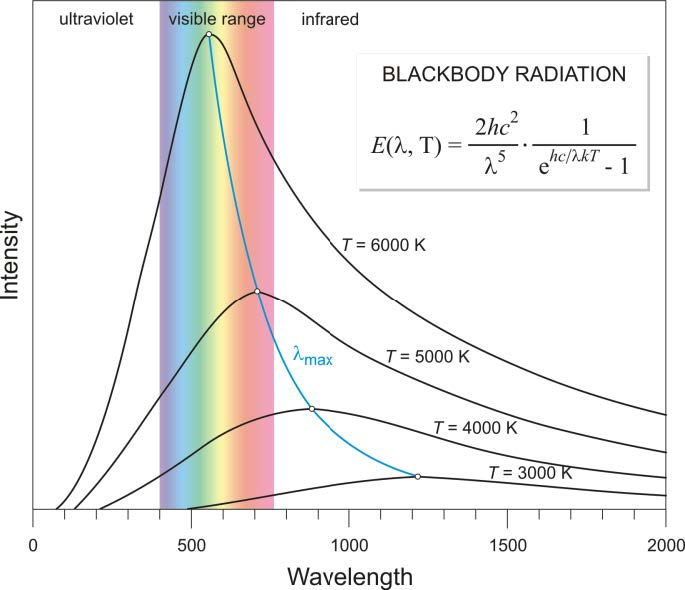
\includegraphics[width=6cm]{files/img1}
\end{center}

\begin{enumerate}[label=\alph*.]
    \item Calcule el potencial eléctrico a lo largo del eje $z$ y deduzca el valor de la densidad superficial de carga $\sigma$
    como función de $V_0$ y $a$. Ayuda: considere el disco como un conjunto infinito de anillos concéntricos.
    \item Calcule el campo eléctrico en un punto del eje $z$ sabiendo que $z > 0$.
    \item Suponga ahora que se coloca un segundo disco (B) de radio $b$ $(b \ll a)$, de espesor $e$ $(e \ll b)$ y densidad $\rho$
    de tal forma que el centro del disco (B) está prácticamente confundido con el origen. Este disco es libre
    de moverse en el eje $z$. Ambos discos están inicialmente en contacto eléctrico (de forma que la densidad
    superficial de carga es la misma en los dos discos). Determine el valor $V_s$ de la tensión umbral a partir la
    cual se produce el despegue del disco que está encima. Asuma que la aceleración de la gravedad es $g$.
\end{enumerate}

Ayuda. Utilice el siguiente resultado: $\int \frac{x}{\sqrt{a^2 + x^2}}\;dx = \sqrt {a^2 + x^2}$

\vspace{20px}
\textit{Solución:}
\\



\textbf{a}. El potencial debido a una distribución continua de carga puede calcularse eligiendo un elemento de carga $dq$ que puede considerarse
como una carga puntual, y tomando en consideración el principio de supersición, el potencial se obtiene mediante la integral:

\begin{equation*}
    V = \int \frac{k\;dq}{r}
\end{equation*}

Consideramos el disco como un conjunto infinito de anillos concéntricos.
Tenga un anillo radio $b$ y carga $Q$. Un elemento de carga $dq$
de este anillo está a la distancia $r = \sqrt{z^2 + b^2}$ de un punto $P$ situado en el eje $z$. Esta distancia es la misma para todos
los elementos de carga del anillo, por lo que el potencial en el eje del anillo es:


\begin{equation*}
    V = \frac{k}{\sqrt{z^2 + b^2}} \int dq = \frac{k\;Q}{\sqrt{z^2 + b^2}}
\end{equation*}

Suponemos ahora que el disco posee una carga total $Q$ distribuida uniformemente sobre su superficie. Si $\sigma = Q / (\pi a^2)$ es la densidad
superficial de carga del disco, la carga de un anillo concéntrico es $dq = \sigma 2\pi b\;db$.
El potencial calculado para el anillo
concéntrico se expresa ahora como un elemento diferencial:


\begin{equation*}
    dV = \int \frac{k\sigma 2\pi b\;db}{\sqrt{z^2 + b^2}}
\end{equation*}

Integrado desde $b = 0$ hasta $b = a$:

\begin{equation*}
    V = 2\pi k \sigma \left(\sqrt{z^2 + b^2}\right) \Big|_0^a =  2\pi k \sigma \left( \sqrt{z^2 + a^2} - \sqrt{z^2} \right)
    = 2\pi k \sigma |z| \left( \sqrt{1 + \frac{a^2}{z^2}} - 1 \right)
\end{equation*}


Considerando que $V_0 = V(z = 0)$, el valor de la densidad superficial de carga $\sigma$ en función de $V_0$ y $a$ es:

\begin{equation*}
    \sigma = \frac{V_0}{2\pi k a}
\end{equation*}

\vspace{20px}

\textbf{b}. La diferencia de potencial es la variación de energía potencial por unidad de carga asociada al desplazamiento $d \vec{\math{\ell}}$ ante
la fuerza eléctrica que sufre la carga por la presencia de un campo eléctrico: $dV = - \vec{E} \cdot d\vec{\ell}$.\\

Por simetría, el campo generado por el disco en un punto $P$ del eje $z$ solo tiene una componente en la dirección del eje $z$. Podemos calcular entonces
$E_z = - dV / dz$. Considerando $z > 0$:

\begin{equation*}
    E_z = 2\pi k \sigma \left[ \frac{1}{2}(z^2 + a^2)^{-1/2})2z -1 \right] = 2\pi k \sigma \left( 1 - \frac{z}{\sqrt{z^2 - a^2}} \right)
\end{equation*}


\vspace{20px}

\textbf{c}. En este apartado debemos encontrar el módulo de la fuerza eléctrica que repele el disco (B) hacia arriba, y que contrarresta su peso
$mg$, o en función de la densidad, $\rho \pi b^2 e g$.\\

Los dos discos comparten densidad superficial de carga, por lo que la carga total del disco (B) se puede expresar como $Q_B = \sigma \pi b^2$.
En el apartado anterior, calculamos que en el punto de la superficie del disco (A) en el eje $z$, el campo eléctrico es $E_z = 2 \pi k \sigma$.\\

Por todo ello, podemos expresar la fuerza eléctrica que ejerce el disco A sobre el disco B como:

\begin{equation*}
    F_{AB} = Q_B\,E_z = \sigma \pi b^2 \;2 \pi k \sigma = 2 \pi^2 k \sigma^2 b^2
\end{equation*}

Utilizando el resultado del apartado a. podemos expresar esta fuerza en función de la tensión $V_0$:

\begin{equation*}
    F_{AB} = \frac{b^2}{2ka^2}\;V_{0}^2
\end{equation*}

Sustituyendo $V_0$ por $V_s$ e igualando esta expresión al peso del disco, podemos obtener
la tensión umbral $V_{s}$ a partir de la cual se produce el despegue:


\begin{equation*}
    \frac{b^2}{2ka^2}\;V_{s}^2 = \rho \pi b^2 e g \quad \Rightarrow \quad
    V_{s}^2 = 2 \pi k a^2 e \rho g  \quad \Rightarrow \quad
    V_s = a \sqrt{2 \pi k e \rho g}
\end{equation*}

Realizando un análisis dimensional de la última expresión, obtenemos:

\begin{equation*}
    m \; \sqrt {\frac{N \cdot m^2} {C^2} \; \frac{Kg}{m^3} \;  m  \; \frac{m}{s^2}} =
    m   \; \sqrt \frac{N^2}{C^2} = V
\end{equation*}

por lo que la solución es dimensionalmente correcta.\\

Además, observamos que la solución no depende del radio $b$ del disco (B),
que puede considerarse como una carga puntual ya que $b \ll a$. La solución sí que depende del radio $a$ del disco (A), que
da una medida de la fuerza del campo eléctrico generado por el disco (A), y del espesor $e$ y la densidad $\rho$ del disco (B),
que influyen en el peso que debe contrarrestrar la fuerza eléctrica de repulsión entre los dos discos.
